\section{Evaluation}
\label{sec:evaluate}

Our platform has been actively deployed for over a year, bringing the benefits of a safe programming environment for MCUs to hundreds of thousands of active users. In this section we provide a broad, quantitative evaluation of the cost at which these benefits are realized. We do this with several micro-benchmarks that give insight into the performance of \MC and \CO across the Uno, micro:bit, and CPX devices. We break down results by layer (\CO and \MCN) to give an insight into how each performs.

\subsection{Benchmarks, Devices, and Methodology}

To analyze the performance of our solution, we have written a suite of programs to evaluate different aspects of \MC and \CO  on a representative selection of real hardware devices. Throughout, we use the C++ \CO benchmarks as a baseline; the STS benchmarks show the overhead added by \MCN. These programs were written in both C++ and STS, and evaluated on the three devices listed in Table~\ref{table:devices}: The micro:bit (Nordic nRF51 MCU), the CPX (Atmel ATSAMD21 MCU), and the Uno (Atmel ATmega MCU).

The Uno is the simplest of these devices,
consisting of an 8-bit processor running at 16 MHz, with only 2kB of RAM and 32kB of flash.
The micro:bit has a 32-bit Cortex-M0 clocked at 16MHz, with 16kB RAM and 256kB of flash. The CPX is a 32-bit Cortex-M0+, which offers greater energy efficiency and performance; it clocks at 48 MHz, has 32kB of RAM and 256kB of flash. The Uno and micro:bit \MC targets use the untagged compilation strategy, while the CPX target uses the tagged strategy (see Section~\ref{sec:untagged-tagged}). The benchmarks are classified into two types, each with their own methodology:

\begin{enumerate}
    \item \textit{Performance Analysis}: Tests that capture time taken to perform a given operation. For these benchmarks, we toggle physical pins on the device at key points in
    the test code. We then measure the time to
   execute the operation, by using a calibrated oscilloscope observing these pins. This allows us to derive highly accurate real time
   measurements without biasing the experiment.

    \item \textit{Memory Analysis}: Tests that capture the RAM or FLASH footprint of a certain operation. A map of memory is logged before and after the execution of an operation, allowing us to compute the cost.
    A serial terminal captures the output of these tests.
\end{enumerate}

Note that memory and performance analysis are done in separate runs
to ensure logging does not affect time-related measurements.

\subsection{Tight Loop Performance}

To place the performance of \MC in context, we perform a comparative evaluation of \MC against two state-of-the-art
solutions adopted by educators in the classroom, using native C++ as our baseline. The two points of comparison are MicroPython~\cite{MicroPython}, an implementation of Python for MCUs, and Espruino~\cite{espruinoBook}, an implementation of JavaScript for MCUs. For the CPX, a fork of MicroPython known as ``CircuitPython'' was used. Both MicroPython and Espruino use virtual machine (VM) approaches.

To give an indicative general case execution time cost of each solution, we created a simple program that counts from 0 to 100,000 in a tight loop in each solutions' respective language; the results are shown in Table~\ref{table:vm-comparison}. On AVR we count to 25,000 (to fit within a 16 bit \texttt{int}) and scale up the results.

For MicroPython and Espruino on the micro:bit, the run is \emph{two or more orders of magnitude slower} than a native \CO program.
\MC performs only 2x slower. The slowdown reflects the simple code generator of our STS compiler. It should be noted that \MC for the CPX uses the tagged approach, which allows for seamless runtime switching to floating point numbers, resulting in a further 3x slowdown. For both devices, we can observe that \MC outperforms both the VM-based solutions of MicroPython and Espruino by at least an order of magnitude.

MicroPython and similar environments cannot run on the Uno due to flash and RAM size limitations. We also ran into these limitations, and as a result, developed two compilation modes for AVR. One compiles STS to AVR machine code, and the other (\MC VM) generates density-optimized byte code for a tiny ({\textasciitilde}500 bytes of code) interpreter. The native strategy achieves code density of about 60.8 bytes per statement, which translates into space for 150 lines of STS user code. The VM achieves 12.3 bytes per statement allowing for about 800 lines. For comparison, the ARM Thumb code generator used in other targets achieves 37.5 bytes per statement, but due to the larger flash sizes we did not run into space issues.

\begin{table}[]
    \centering

    \begin{tabular}{c|c|c|c|}
    \cline{2-4}
    \multicolumn{1}{l|}{}             & UNO    & micro:bit & CPX   \\ \cline{1-4}
    \multicolumn{1}{|c|}{\CO}         & 171ms  & 102ms     & 31ms  \\ \hline
    \multicolumn{1}{|c|}{\MC}         & 2.4x   & 2.1x      & 7.3x  \\ \hline
    \multicolumn{1}{|c|}{\MC VM}      & 15.3x  & -         & -     \\ \hline
    \multicolumn{1}{|c|}{MicroPython} & -      & 101x      & 183x  \\ \hline
    \multicolumn{1}{|c|}{Espruino}    & -      & 1139x     & -     \\ \hline
    \end{tabular}
    \caption{\label{table:vm-comparison} A comparison of execution speed between: native C++ with \CON; \MC compiled to native machine code; \MC compiled to AVR VM; MicroPython; and Espruino. The first line lists the C++ time, while subsequent lines are slowdowns with respect to the C++ time. The 6.4x slowdown of \MC VM compared to native \MC on the Uno is compensated with 5x better code density.}
    \vspace{-20pt}
\end{table}


\subsection{Context Switch Performance}

\begin{figure}[ht]
    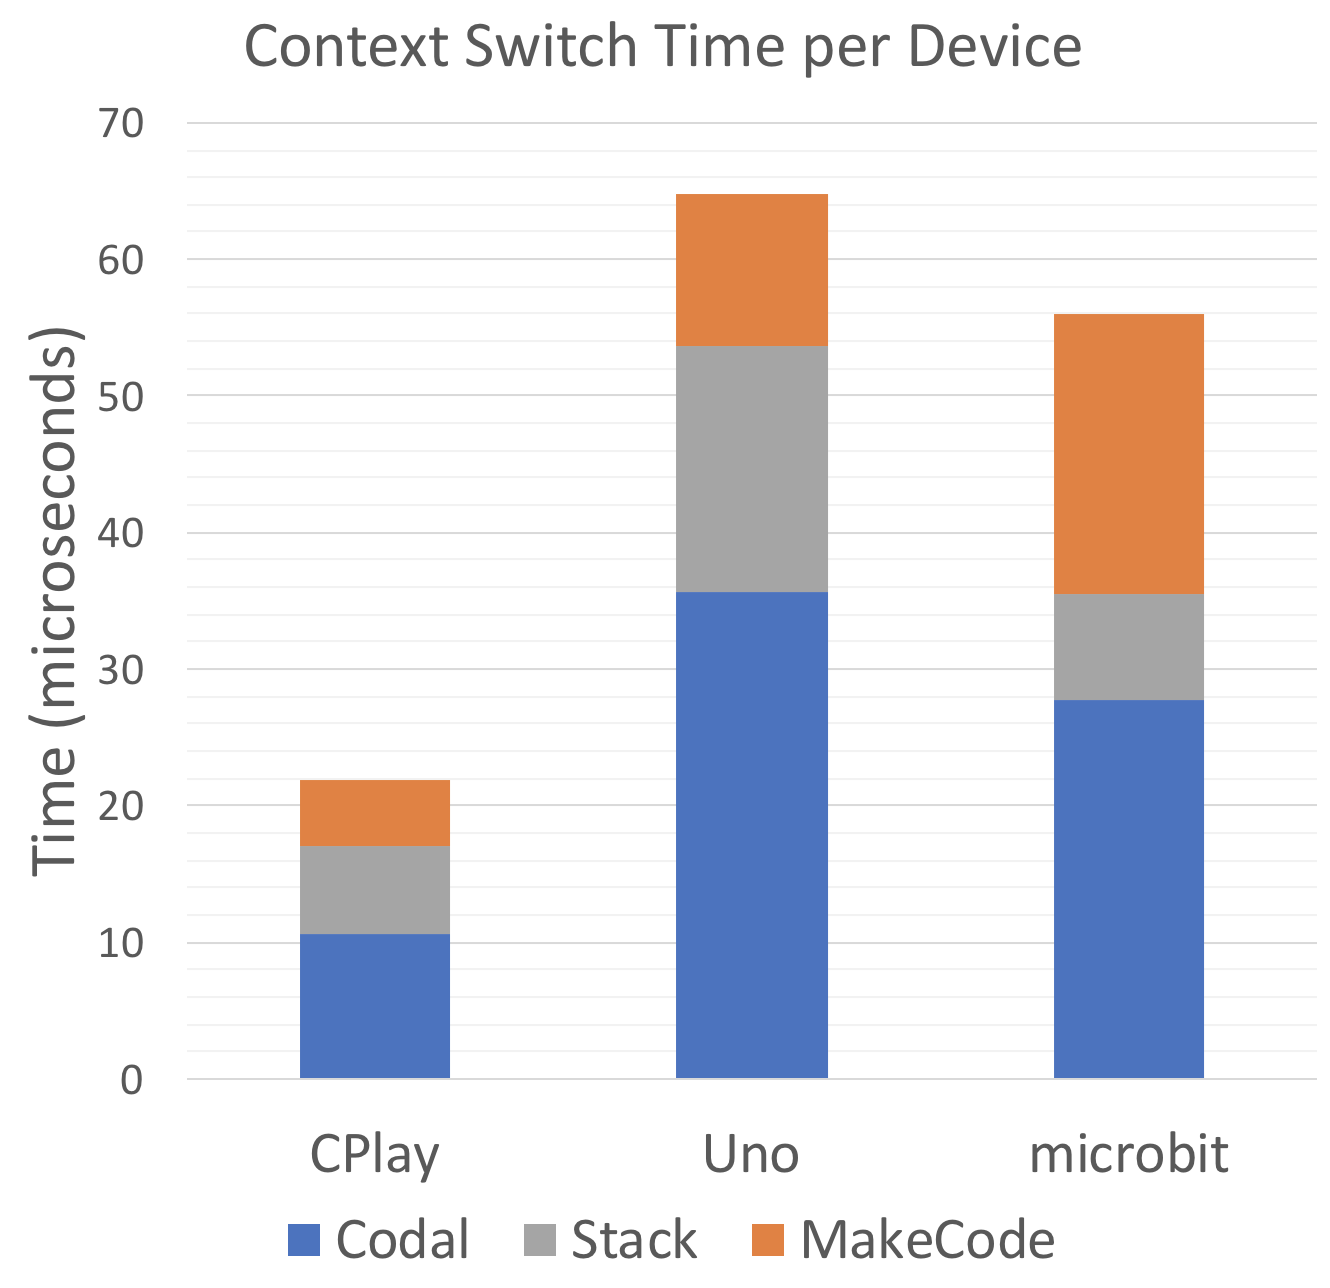
\includegraphics[width=.8\columnwidth]{images/context-switch.png}
\caption{\label{fig:context-switch}Base context switch profiles per device.}
\end{figure}

\begin{figure}[ht]
    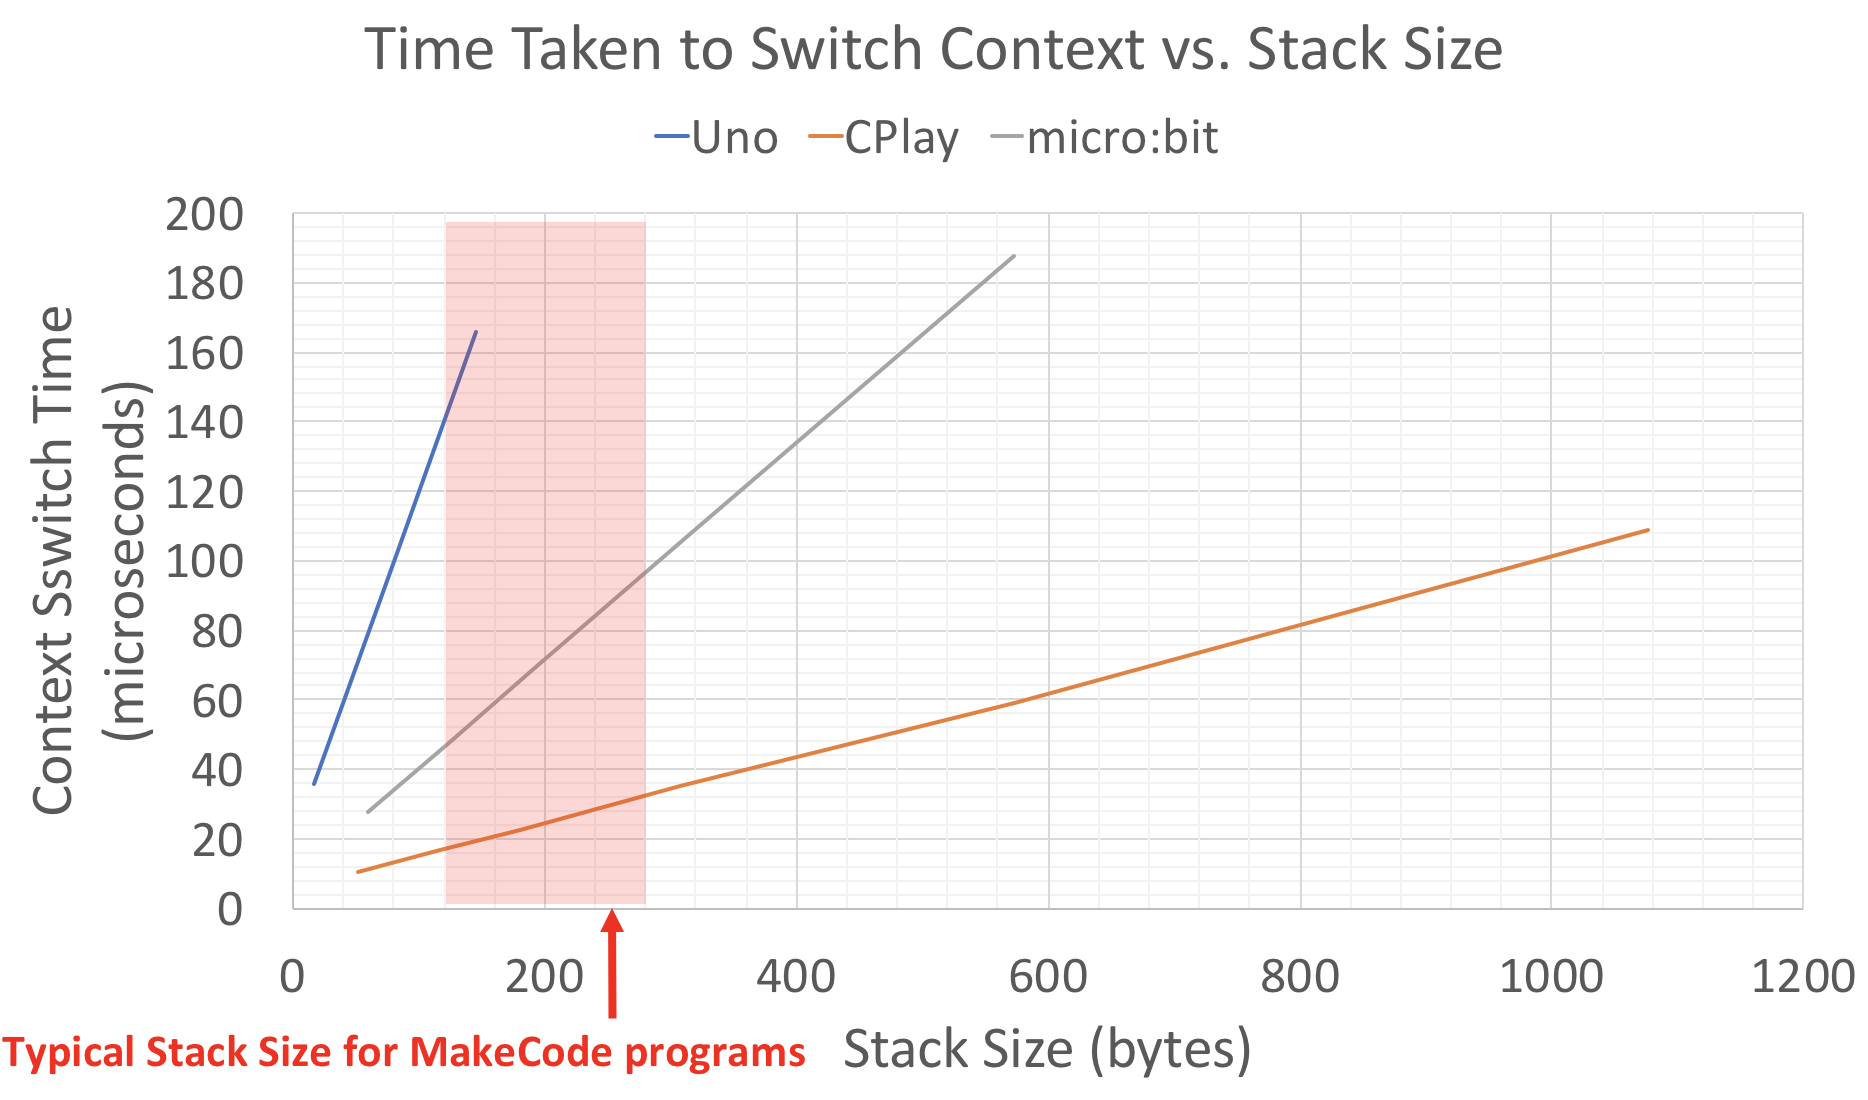
\includegraphics[width=\columnwidth]{images/context-vs-stack.png}
\caption{\label{fig:context-vs-stack}Time taken to perform a context switch against stack size.}
\end{figure}

To evaluate the performance of \CON's scheduler we conducted a test that created two fibers, continuously swapped context, and measured the time taken to complete a context switch.
We performed this test in both STS and C++ and the resulting profiles can be seen in Figure~\ref{fig:context-switch}, which
breaks the context switch down into three phases:
(1) \CON, the time it takes to perform a context switch in \CON;
(2) Stack, the time taken to page out the \MC stack; and
(3) \MCN, the overhead added by \MCN.

From these results, we observe that context switches generally take tens of microseconds. The cost of \CON's stack paging approach can also be a significant, but not dominant cost. The cost of stack paging would of course grow with stack depth. Figure~\ref{fig:context-vs-stack} profiles the time a context switch takes with an increasing stack size across all three devices in \CON. This is similar to the previous test, except we placed bytes (in powers of 2) on the stack of each fiber, starting from 64 and finishing at 1024. The difference in gradients, and ranges of values can be put down to device capability. For instance, the Uno has an 8-bit word size, which means more instructions are required to copy the stack, this results in a steeper gradient than the other two devices. The vertical band indicates typical stack sizes for \MC programs based on a representative set of examples.

%For the uno, the context switch profile is for the native implementation only.

\subsection{Performance of Asynchronous Operations}

To gauge the cost of asynchronous operations in \CON, we tested three commonly used code paths, designed to determine the efficiency of \CON's \emph{fork-on-block} Asynchronous Procedure Call (APC) mechanism that underpins all event handlers in \MC and \CON. We measured the RAM and processor cost of: (1) creating a fiber; (2) handling a non-blocking APC call; and (3) handling a blocking APC call. We used the CPX for this experiment.

Non-blocking APC calls, the best case, have a small overhead of 32 bytes of RAM and 4.01 microseconds of processing time. Blocking APC calls, the worst case, incur a large overhead of 204 bytes of RAM and 32.4 microseconds of processor time. Creating a fiber costs 136 bytes of RAM and 35.4 microseconds of processing time. These results highlight the performance gains of the opportunistic fork-on-block mechanism over a naive approach that would execute every event handler in a separate fiber.

\subsection{Flash Memory Usage}

\begin{table}[t]
\centering
\begin{tabular}{c|c|c|c|}
\cline{2-4}
                                                                                                & CPX & micro:bit & Uno  \\ \hline
\multicolumn{1}{|c|}{\MC}                                                                       & 20.46 & 12.14     & 7.79 \\ \hline
\multicolumn{1}{|c|}{\CO}                                                                       & 29.85 & 34.35     & 13.7 \\ \hline
\multicolumn{1}{|c|}{\begin{tabular}[c]{@{}c@{}}Supporting Libraries\end{tabular}} & 14.99 & 24.28     & -    \\ \hline
\multicolumn{1}{|c|}{C++ Standard Library}                                                     & 43.14 & 24        & 1.03 \\ \hline
\end{tabular}

\caption{\label{table:flash-consumption}
Flash consumption of a \MC binary~(kB)}
\vspace{-25pt}
\end{table}

MCUs make use of internal non-volatile FLASH memory to store program code. Table~\ref{table:flash-consumption} shows the per device flash consumption of each software library used in the final \MC binary. To obtain these numbers, we analyzed the final map file produced after compilation. The ordering of the table aligns with the composition of the software layer: \MC builds on \CO which builds on the C++ standard library and supporting libraries.
\MC and \CO consume 108 kB of flash, whereas CircuitPython consumes 201 kB, MicroPython consumes 228 kB, and Espruino consumes 142 kB of flash.
This means that users can write sizeable applications in \MCN, without the worry of running out of flash memory.

From the bottom up, the profile of the standard library changes dramatically for each device: The Uno has a very lightweight standard library; the micro:bit uses 64-bit integer operations (for timers) which requires extra standard library functions; and the CPX requires software floating point operations pulling in more standard library functions.

The size of \CO and \MC scales linearly with the amount of functionality a device has, due to the component oriented nature of \CO and transitively \MCN. For instance, the Uno has few onboard components when compared to the CPX and micro:bit. The modular composition of \CO allows us to support multiple devices with a variety of feature sets, while maintaining the same API at the \MC layer.

\subsection{RAM Memory Usage}

\begin{table}[t]
\centering
\begin{tabular}{c|c|c|c|}
\cline{2-4}
                                                                                                & CPX & micro:bit & Uno   \\ \hline
\multicolumn{1}{|c|}{\MC}                                                                       & 0.612 & 1.069     & 0.074 \\ \hline
\multicolumn{1}{|c|}{\CO}                                                                       & 0.369 & 0.214     & 0.156 \\ \hline
\multicolumn{1}{|c|}{\begin{tabular}[c]{@{}c@{}}Supporting Libraries\end{tabular}} & 0.312 & 0.923     & -     \\ \hline
\multicolumn{1}{|c|}{C++ Standard Library}                                                     & 0.161 & 0.149     & 0.074 \\ \hline
\end{tabular}
\caption{\label{table:ram-consumption}Static RAM consumption of a \MC binary~(kB)}
\vspace{-20pt}
\end{table}

Table~\ref{table:ram-consumption} shows the per device RAM consumption of each software library used in the final \MC binary. To obtain these numbers, we analyzed the final map file produced after compilation. At runtime, \MC dynamically allocates additional memory: 1.56 kB for the CPX, 560 bytes for the micro:bit, and 644 bytes for the Uno. We also can see that in all cases, the RAM consumption of \MC and \CO is well within the RAM available of each device.

\MC and \CO consume a small amount of resources in comparison: CircuitPython (a derivative of MicroPython) consumes 12.8~kB, MicroPython consumes 9.5~kB, and Espruino consumes 5.3~kB of RAM. On the micro:bit, the Bluetooth stack requires 8~kB of RAM to operate. Due to MicroPython's RAM consumption this means that Bluetooth is inoperable. Comparatively, Espruino does enable the Bluetooth stack, but users have just \textasciitilde300 bytes available for their programs due to the overhead incurred.

% Add globals maps and profile of listener and fiber.

% The CPX runtime is the largest, as the CPX device has lots of on-board
% components, and this runtime shares much of its code with other SAMD21 \MC targets.
% The compiled C++ runtime is 114k in total, with \CO accounting for 29k, with an
% additional 15k from libmbed. The \MCN-common-packages adds 20k, and also in
% an additional 49k of math support libraries (floating point operations,
% including trigonometry and number printing/parsing).
% As the SAMD21 has 256k of flash, we did not worry about optimizing this runtime for space.

% On the Uno, which has 32k of flash, the much \MC runtime is 8k and \CO is 14k (since
% the Uno only requires basic GPIO, i2c and serial drivers), leaving 10k for user code.

% The TypeScript part of the runtime is 1060 statements on the CPX and 216 on the Uno.
% In our microbenchmarks, 99\% of that runtime is tree-shaken away.

\subsection{Compiling Static TypeScript}

During compilation, the entire STS program (including the STS runtime) is passed to the TypeScript (TS) language service for parsing. Then, only the remaining part of the program (after code shaking) is compiled to native code. On a modern laptop, using Node.js, TS parsing and analysis takes about 0.1ms per statement, and \MC compilation to native code takes about 1ms per statement.
While the TS compiler has been optimized for speed, \MCN's native compilation process has not. For example, the CPX TS pass is dominated by compilation of the device runtime and takes about 100ms, whereas the \MC pass typically only includes a small user program and a small bit of the runtime, resulting in less than 100ms. Thus, compilation times are under 200ms for typical user programs of 100 lines or less.

\subsection{Extensibility}

% I think 'processor' could be understood as generic ARM or generic AVR, not a specific MCU with peripherals
Adding a new device in \CO is trivial once a MCU has been ported. The porting of a MCU is where we observe the largest development overhead, as low-level implementations of drivers for I2C, Serial, and SPI may have to be re-written. Due to \CON's abstraction model, once low-level drivers have been implemented, drivers for higher level components like Accelerometers (which depend on high-level interfaces for low-level drivers) can be immediately adopted if hardware is present. A similar technique is used in \MC for simulators.

% Not really a result, more of a description of design, with an anecdotal comment about speed.

% should be moved further up and described alongside AVR VM vs. Native

% The AVR VM was specifically designed for high code density, since \CO
% leaves less than 10k for TS runtime and user code on the Uno. The interpreter is implemented in assembly, always included with the program, and is around 0.5k.
% There are about 30 opcodes, some of which can take 1 or 2 byte arguments. There are also a few combined opcodes, representing a sequence of one argument-less opcode, and one with an argument, which improves code density by about 25\%. Opcodes are direct offsets into the code of the interpreter, speeding up execution. They operate on a stack (mainly for function calls) and a special scratch register. There is essentially no stack space overhead compared to native AVR compilation. The speed overhead is around 4x-5x (with respect to native) for computational tasks.


%\subsection{Implementation}
% •	\CO (SAMD21 and AVR): base runtime (C++ only)
% •	pxt
% •	pxt-common-packages: C++ and Static TypeScript
% •	pxt-adafruit
% •	pxt-arduino-uno
% •	pxt-monaco, pxt-blockly

%mmoskal [10:10 AM]
%`pxt checkdocs --snippets --re perf --stats`
% [10:11]
% I compile empty sample first twice, to reduce JIT costs
% [10:12]
% also, the first "compile prep" is slightly more costly, since it parses a hex file
